\documentclass[twocolumn]{article}
\usepackage[
    a4paper,
    top=0.75in,
    bottom=1in,
    left=0.7in,
    right=0.7in
]{geometry}
\usepackage{graphicx}
\usepackage{algpseudocode}
\usepackage{amsmath}
\usepackage{amssymb}
\usepackage{tabularx}
\usepackage{courier}
\usepackage{hyperref}
\usepackage{algorithm}
\usepackage{booktabs}
\usepackage{etoolbox}
\usepackage{placeins}
\usepackage{subcaption}
\usepackage{afterpage}
\usepackage{cuted}
\usepackage{capt-of}
\usepackage{titlesec}

\setlength{\floatsep}{6pt plus 2pt minus 2pt}
\setlength{\textfloatsep}{8pt plus 2pt minus 2pt}
\setlength{\intextsep}{6pt plus 2pt minus 2pt}
\setlength{\dblfloatsep}{6pt plus 2pt minus 2pt}
\setlength{\dbltextfloatsep}{8pt plus 2pt minus 2pt}
\captionsetup{font=footnotesize,skip=3pt}
\titlespacing*{\section}{0pt}{1.0ex plus 0.2ex minus 0.1ex}{0.6ex plus 0.1ex}
\titlespacing*{\subsection}{0pt}{0.9ex plus 0.2ex minus 0.1ex}{0.4ex plus 0.1ex}
\AtBeginEnvironment{thebibliography}{%
    \scriptsize
    \setlength{\itemsep}{0pt}
    \setlength{\parskip}{0pt}
    \setlength{\parsep}{0pt}
}

\title{\vspace{-2cm}The Effect of Induction Head Ablation on Repetition Dynamics in Large Language Models}
\author{Arjun Rao}

\date{May 2026}

\begin{document}

\maketitle

\begin{abstract}
    This study aims to examine the effects of ablating top induction heads on entropy and local repetition in the output of a transformer. In the GPT-2 Small model, we find that global top induction head ablation leads to greater repetition in text output. This finding indicates the potential role of induction heads in preventing model failure in autoregressive models. Additionally, we find a negative correlation between $\Delta$Entropy and induction head ablation, indicating that greater local repetition is not a product of lower entropy in logits. We also find induction head ablation to have a similar, albeit lesser, effect on a larger model like GPT-2 Medium. Overall, these findings advance our understanding of the inner workings of these models.      
\end{abstract}

\section{Introduction}

Induction heads are a circuit in transformers that contribute to in-context learning by copying and completing sequences that have occurred before. These attention heads enable predictions of the form \texttt{[A] $\xrightarrow[]{}$ [B]}, given that \texttt{[A][B]} exists in the training sequence. Olsson et al. demonstrated the existence of induction heads and their effect across a range of simple attention-only models, as well as more complex models that contain both attention heads and Multi-Layer Perceptrons (MLPs) \cite{olsson2022incontextlearninginductionheads}. This inductive behavior of attention heads can be understood through the ability of each individual attention head to determine an attention score, which determines the tokens to which a particular token should attend. This attention score, quantifying the extent to which token $i$ draws from token $j$, is defined in \ref{eq:attentionscore}

\begin{equation}
    S_{ij} = r_i W_Q W_K^T r_j
    \label{eq:attentionscore}
\end{equation}

where $r_i$ and $r_j$ represent token embeddings, and $W_Q$ and $W_K$ represent the randomly initialized weights of the Query and Key matrices, respectively. While the attention score determines which other tokens a particular token should attend to, it is the $W_O$ (output matrix of the attention head) and $W_V$ (value matrix) that determine the extent to which attention scores impact logit probabilities. With regard to induction, existing literature establishes that $W_{OV}$ and $W_{KV}$ tend to draw on tokens equivalent to the source token, thus creating this induction behavior \cite{elhage2021mathematical}. \\

The exact mechanism by which these induction heads enable in-context learning is poorly understood. However, what is interesting is that they are able to preserve induction without becoming trapped in a feedback loop whereby they repeat existing information. Repetition is a well-known failure mode in autoregressive and recurrent language models that is often attributed to greedy decoding, where the model temperature is set to 0 or otherwise maintained at a low level. This stifles creativity in a model's output and prevents overall semantic understanding by the transformer. This behavior is not commonly seen in modern LLMs, thus leading to a valid research question in mechanistic interpretability regarding how LLMs largely overcome this failure mode. This line of inquiry could also help further reduce the few instances in which transformers enter repetition loops, thereby improving model performance as well. \\

To understand repetition dynamics, this study aimed to examine induction heads. The choice to examine induction heads was motivated by empirical observations while studying performance differences between models and induction head-ablated models. In conversation with these models, induction head-ablated models tended to repeat tokens from the input prompts, while original models were more creative in their output. This study aims to rigorously test these observations across different prompts and models and attempt to understand the underlying mechanisms by which repetition occurs in ablated models.

\section{Methodology}

\subsection{Method for Determining Induction Heads}

Induction heads for the models used in this study were determined using an algorithm to compute an induction score to determine whether model predictions align with the sequence through which the transformer performs a forward pass. A random matrix $S \in \mathbb{R}^{L \times H}$ of 50 token embeddings is initialized, and a forward pass is performed after each token in $S_R$ given the input $\{ S_1, S_2 \dots S_{R_1}, S_{R_2} \dots\}$ to test induction behavior. An induction score (see Equation \ref{eq:inductionscore}) is computed based on the prediction at every head ($h$), comparing the attention probabilities given token $t$ with the expected token at position $p_{t+1}$ across $b$ batches and $N$ sequences. An induction score threshold of 0.5 was selected for determining top induction heads in experiments with the GPT-2 Small transformer. 

\begin{equation}
    InductionScore(h) = \frac{1}{N}\sum A_{b,h,t,p_{t+1}}
    \label{eq:inductionscore}
\end{equation}

\begin{table*}[t!]
\centering
\footnotesize
\renewcommand{\arraystretch}{1.15}
\setlength{\tabcolsep}{4pt}
\setlength{\abovecaptionskip}{0.25em}
\setlength{\belowcaptionskip}{0.4em}


\begin{tabular}{p{3cm} p{5.5cm} p{5.5cm}}
\toprule
\textbf{Category} & \textbf{Prompt 1} & \textbf{Prompt 2} \\
\midrule

Factual Knowledge &
\texttt{The capital of India is} &
\texttt{The largest planet in the solar system is}
\\[0.35em]

Narrative Completion &
\texttt{Once upon a time there was} &
\texttt{In a distant galaxy humanity discovered}
\\[0.35em]

Reasoning &
\texttt{The reason climate change is difficult to solve is} &
\texttt{Artificial intelligence may become dangerous if}
\\[0.35em]

Inductive &
\texttt{Alice went to Paris. Bob went to London. Alice went to} &
\texttt{The cat sat on the mat. The dog sat on the}
\\[0.35em]

Philosophical &
\texttt{The true meaning of life is} &
\texttt{Materialistic wealth is not sufficient}
\\

\bottomrule
\end{tabular}
\caption{Prompt Categories Used for Analysis}
\label{tab:prompt_categories}
\end{table*}

\subsection{Metrics for Entropy and Local Repetition Rate}

For causal experiments to understand the nature of local repetition in model output and the factors contributing to it, this study determines two metrics: Local Repetition Rate (LRR) and entropy. LRR was selected over existing metrics such as self-BLEU, as the focus of the study is to understand local repetition as opposed to global patterns in token generation. Emphasis was placed on local repetition due to the underlying mechanism of induction heads and to more clearly present transformer traits that might otherwise become obscured in larger token samples. LRR (see Equation \ref{eq:lrr}) measures the frequency of already seen tokens ($w$) within a particular window size ($N$). A window size of 20 was chosen, as we believe it offers a sufficient sample to understand generation dynamics while preserving locality.  

\begin{equation}
LRR = \frac{1}{N} \sum_{i=w+1}^{n} x_i \in \{x_{i-w} \dots x_{i-1}\}
\label{eq:lrr}
\end{equation}

To better understand local repetition, model entropy was also studied, which serves as a proxy for creativity in a model's logits. In the context of mechanistic interpretability, entropy is used to measure the degree of randomness in the softmax probabilities derived from logits ($p_i$). Equation \ref{eq:entropy} gives the process used to calculate predictive entropy from the final output distribution in the transformer architecture used in this study.

\begin{equation}
    H = -\sum p_i \log p_i
    \label{eq:entropy}
\end{equation}



\subsection{Experiments comparing Original and Ablated Models}
\label{sec:2.3}

Multiple pipelines have been used in this study to better understand the contribution of individual heads to the repetitive behaviors being studied. To first understand entropy dynamics prior to studying LRR, the simple factual prompt \texttt{"The Capital of India is"} was selected. For this demo prompt, $\Delta$Entropy was calculated by subtracting the final layer entropy of the model where significant heads ($InductionScore(h) > 0.5$) were ablated from original model entropies. This $\Delta$Entropy was computed for the same demo prompt by ablating each head individually as opposed to the global ablation performed in the first experiment. The goal of this experiment was to establish a baseline to understand repetitive dynamics using standard metrics such as Shannon entropy as opposed to using specific case-defined metrics like LRR. Empirical observation had led to the hypothesis that ablating induction heads leads to greater repetition, and these two experiments with entropy contribute to understanding whether induction heads might, in some ways, make models more creative in their outputs. \\



Having established a baseline through entropy testing, the focus next shifted to statistically validating the main hypothesis regarding Local Repetition. For this, 10 prompts, listed in Table \ref{tab:prompt_categories}, belonging to different categories were chosen. For all LRR experiments, a maximum of 100 tokens was generated for all the input prompts. The range of prompt categories, from testing factual recall to inductive behavior to more open-ended questions, in addition to ensuring generalization of the hypothesis, serves the additional purpose of testing inner model behavior for different kinds of input. To quantify the differences between the original and ablated models, $\Delta$LRR was used as the standard criterion. In line with the previous experiment on entropy, this metric was first computed by global ablation of significant heads. It would have been computationally too expensive to compute $\Delta$LRR on a head-by-head basis, so the most open-ended narrative completion prompts were used to better understand individual head contribution to repetitive behavior. \\

To determine whether induction heads in particular were responsible for this local repetition, a 5-instance control trial was performed comparing the results of ablating the top 6 induction heads against 6 randomly selected non-induction heads. This experiment helps to isolate the effects of induction heads over any other attention head in determining repetition dynamics. To generate casual mechanistic insights on the role of induction heads, activation patching was performed for the top induction heads, the details of which are expanded on in \ref{sec:actpatching}. \\

As a final experiment to understand induction head contribution to repetition dynamics, an analysis was conducted comparing global ablation of the top $k$ induction heads and their effect on mean $\Delta$LRR across all prompts. The motivation behind this experiment was to determine whether repetition behavior compounds linearly as more induction heads are ablated or whether there exists a threshold number of induction heads that leads to a significant increase in $\Delta$LRR.


\section{Results}
\subsection{Effects of Ablation on Entropy}

In investigating the effect on final-layer entropy as a result of global top-6 induction head ablation, we determined that there was an increase in model entropy as a result of induction head ablation. The original entropy of the model was 5.82, which increased to 6.40 in the ablated model. This might be attributed to greater variance in logit probabilities and probabilities converging on a single token as opposed to representing greater stochasticity in token probabilities. There is some evidence of this in Table \ref{tab:top_token}, which shows that the ablated model has high confidence in its prediction of \texttt{'India'} to an extent that is not seen in the original model. This convergence of probability might be the causative factor for an increase in entropy. This result is also counterintuitive to an extent in that one would expect model entropy to decrease given that the predicted token already exists in the prompt. But, we believe that the $\Delta H$ value is more a product of the computational factors of entropy as opposed to its characteristic of serving as a proxy for token diversity. \\

\begin{table}[t]
\centering
\footnotesize
\setlength{\tabcolsep}{3pt}
\begin{tabular}{@{}l c l c@{}}
\toprule
\textbf{Original Model} & \textbf{Prob.} & 
\textbf{Ablated Model} & \textbf{Prob.} \\
\midrule
\texttt{home}       & 0.0691 & \texttt{India}      & 0.4744 \\
\texttt{the}        & 0.0681 & \texttt{the}        & 0.1172 \\
\texttt{a}          & 0.0650 & \texttt{now}        & 0.0430 \\
\texttt{now}        & 0.0377 & \texttt{a}          & 0.0326 \\
\texttt{in}         & 0.0245 & \texttt{home}       & 0.0193 \\
\texttt{one}        & 0.0232 & \texttt{Delhi}      & 0.0148 \\
\texttt{known}      & 0.0220 & \texttt{also}       & 0.0107 \\
\texttt{not}        & 0.0185 & \texttt{one}        & 0.0074 \\
\texttt{India}      & 0.0158 & \texttt{not}        & 0.0071 \\
\texttt{being}      & 0.0134 & \texttt{Bangladesh} & 0.0068 \\
\bottomrule
\end{tabular}
\caption{Top predicted token probabilities before and after induction head ablation. There exists a significant difference in the probabilities of the top-2 tokens in the Original and Ablated Model.}
\label{tab:top_token}
\end{table}

Entropy effects of global induction head ablation provide some preliminary results of repetition dynamics which is more rigorously investigated in Section \ref{sec:ableff}. To better understand per-head contributions, $\Delta H$ was calculated by individually ablating each head in the transformer architecture. Figure \ref{fig:delh} represents a heatmap of $\Delta$Entropy by ablating a single head. \\

With regards to individual head contributions, it is observed that all induction head ablations have a positive $\Delta H$, indicating lesser entropy which is consistent with the expectation of repetition in ablated models causing decreased token diversity. It's also worth considering that $\Delta H$ for induction heads present in middle layers does not differ significantly from those of other heads. The only attention heads that have a large individual entropy differential are those in Layer 0, which can be partly explained due to the position of these heads leading to more significant modification to the residual stream. That being said, the particular role of induction heads in entropy or repetition dynamics should not be completely dismissed, as induction circuitry has a far greater impact on model behavior as opposed to the isolated effects of single induction head ablation. This effect is further noticed in comparing the results of individual head ablation and global induction head ablation. Global ablation led to a negative $\Delta H$ while individual head ablation led to a decrease in entropy. This observation broadly aligns with existing literature that global ablation is not the additive sum of individual ablations \cite{nanda2023attribution}.

\begin{figure}[t]
    \centering
    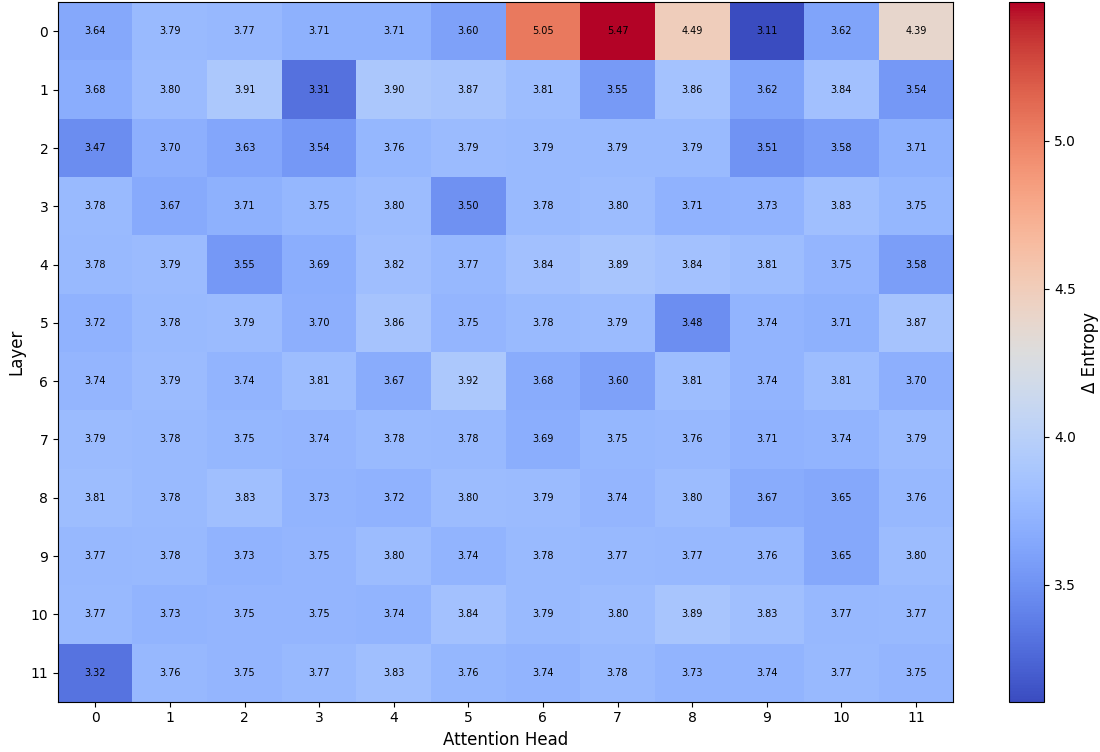
\includegraphics[width=1.0\linewidth]{Figure_1.png}
    \caption{$\Delta H$ computed by ablating each individual head. Few heads in Layer 0 have a significant effect on entropy while most heads contribute to model entropy to a similar extent individually.}
    \label{fig:delh}
   
\end{figure}


\subsection{Ablation effects on LRR}
\label{sec:ableff}
In analyzing the correlation between repetition dynamics and induction head ablation, we first study the $\Delta$LRR of ablating significant heads for the prompts listed in Section \ref{sec:2.3}. The $\Delta LRR$ is likely to be different for different training runs, and to ensure generalization it was ensured that the $\Delta LRR$ remained statistically significant across training runs. For the data reported in Table \ref{tab:delta_lrr}, the one-tailed $p$-value $\approx 1.5 \times 10^{-5}$ which is highly significant. There was no significant difference noted in $\Delta$LRR across prompt categories which contradicts the initial intuition that inductive prompts are likely to have greater local repetition while open-ended prompts would have lesser token repetition. This suggests that local repetition is largely independent of the type of prompt input into the model. \\

While the previous test indicates that induction head ablated models do have greater LRR, it's still necessary to isolate the effect of induction heads as opposed to other attention heads. In the random head-ablation trial conducted, we determined that ablating random heads leads to a very small decrease in local repetition ($\Delta LRR = -0.017$). Figure \ref{fig:dellrr} confirms that induction heads are responsible for this increase in LRR and that it is not a general effect of ablating attention heads.

\begin{table}[!t]
\centering
\scriptsize
\setlength{\tabcolsep}{3pt}
\renewcommand{\arraystretch}{0.94}
\begin{tabular}{@{}p{0.68\linewidth} c@{}}
\toprule
\textbf{Prompt} & $\mathbf{\Delta LRR}$ \\
\midrule
\texttt{The capital of India is} & 0.3605 \\
\texttt{The largest planet in the solar system is} & 0.1348 \\
\texttt{Once upon a time there was} & 0.2644 \\
\texttt{In a distant galaxy humanity discovered} & 0.1462 \\
\texttt{The reason climate change is difficult to solve is} & 0.2222 \\
\texttt{Artificial intelligence may become dangerous if} & 0.3864 \\
\texttt{Alice went to Paris. Bob went to London. Alice went to} & 0.2921 \\
\texttt{The cat sat on the mat. The dog sat on the} & 0.5806 \\
\texttt{The true meaning of life is} & 0.3448 \\
\texttt{Materialistic wealth is not sufficient} & 0.3304 \\
\bottomrule
\end{tabular}
\caption{Difference in Local Repetition Rate ($\Delta LRR$) between original and induction head-ablated models. $\mu_{\Delta LRR} = 0.3062 \pm 0.13$}
\label{tab:delta_lrr}

\end{table}

\begin{figure}[!b]
    \centering
    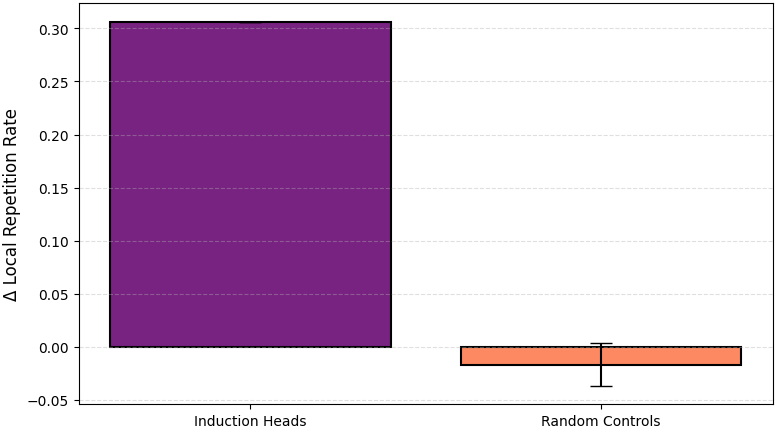
\includegraphics[
width=\linewidth,
height=0.19\textheight,
keepaspectratio
]{Figure_2.png}
    \caption{Induction head ablation leads to greater repetition than random head ablation. The difference in mean $\Delta LRR$ is $0.324$.}
    \label{fig:dellrr}

  
\end{figure}

Similar to the entropy experiments, the next experiment involved determining per-head contributions to LRR. Results of the per-head contribution indicate similarities between per-head $\Delta$LRR and $\Delta H$. Major repetition differences are seen in earlier layers; however, later heads have an insignificant individual contribution. Going by individual head contributions, it can be noted that induction heads do not have a higher LRR contribution than other mid-layer attention heads, which implies that it is the induction circuitry that might be responsible for preventing model failure due to repetition in transformers. The convergence of evidence pointing towards early heads playing an important role in both entropy and repetition dynamics might be a product of earlier heads coding primitive features which cause cascading collapse in later layers \cite{kadem2026interpretingtransformersattentionhead}.

\begin{figure}[!t]
    \centering
    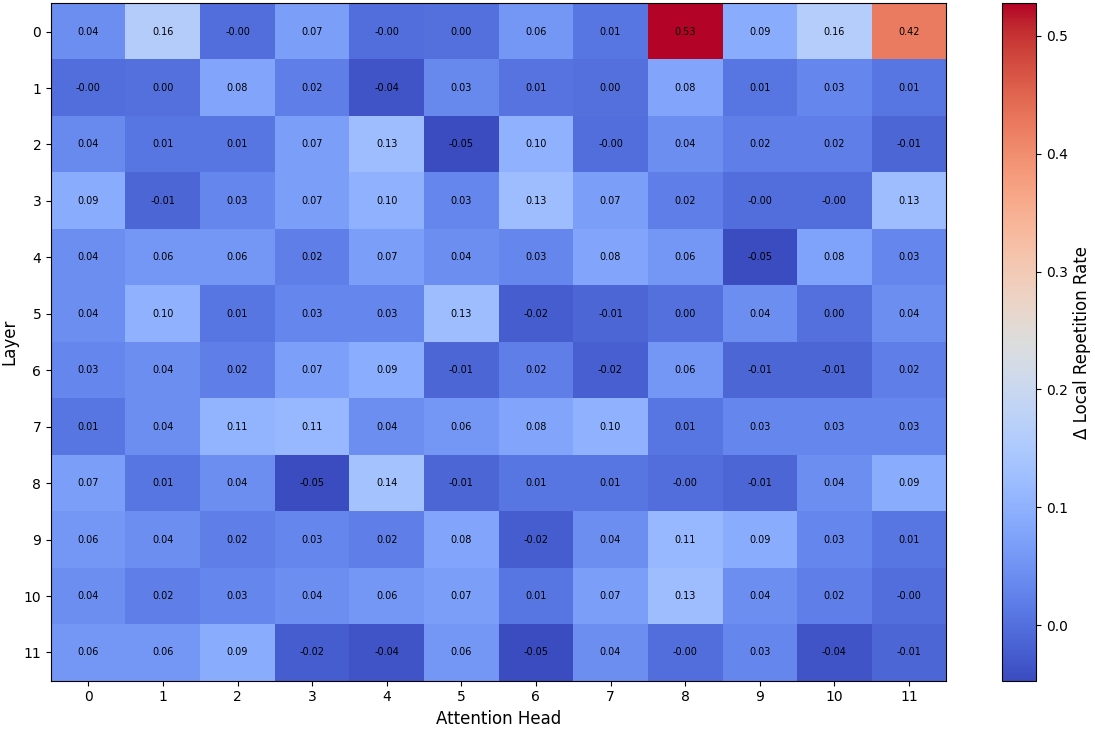
\includegraphics[
width=\linewidth,
height=0.21\textheight,
keepaspectratio
]{Figure_3.png}
    \caption{$\Delta LRR$ computed by individually ablating heads for the prompt \texttt{"Once upon a time there was"}. Individual head ablations produce largely insignificant changes in local repetition.}
    \label{fig:individual_lrr}
\end{figure}

\subsection{Global Activation Patching of Induction Heads}
\label{sec:actpatching}

Activation Patching is a technique to understand the exact contributions of a single component in the transformer by patching the activations of an uncorrupted input into a transformer that is fed the corrupted input to determine the role of that activation in varying model behavior \cite{heimersheim2024useinterpretactivationpatching}. In the context of this study, the activations of the top-6 induction heads of the original model were patched into the ablated model and the LRR of this model's output was compared to that of the original model. This effect was quantified as the recovery rate as defined in Equation \ref{eq:recoveryrate}.

\begin{equation}
    \label{eq:recoveryrate}
    RecoveryRate = \frac{LRR_{patched} - LRR_{ablated}}{LRR_{original}-LRR_{ablated}}
\end{equation}

From this activation patching study, we noted $\mu_{RecoveryRate} \approx 0.965\pm0.15.$ This provides causal mechanistic evidence to suggest that global induction head ablation causes an increase in LRR. On a prompt-to-prompt basis, we find that there is no pattern to note in recovery rate variance with prompt type, which aligns with previous findings that LRR effects are not prompt specific.

\subsection{Non-Linearity in Ablation Effects}

Having determined the effect of induction head ablation on repetition dynamics, we next attempt to identify a relation between the extent of ablation and its impact on LRR. We initially expected that as more heads are ablated there will be an increase in $\Delta$LRR. We were also particularly interested in determining whether there are any non-linear properties to this relation. From a top-$k$ head ablation study, we determined that there is a large increase in $\Delta$LRR after ablating the fourth induction head as seen in Figure \ref{fig:threshold}. The exact value of this threshold number of ablations can vary from trial to trial as we noted in other experiments, but it typically occurs in the range of 3-5 ablations. The interesting factor about this non-linear behavior was that $\Delta$LRR decreased after this threshold number as opposed to plateauing at a certain value. \\

\begin{figure}[!b]
    \centering
    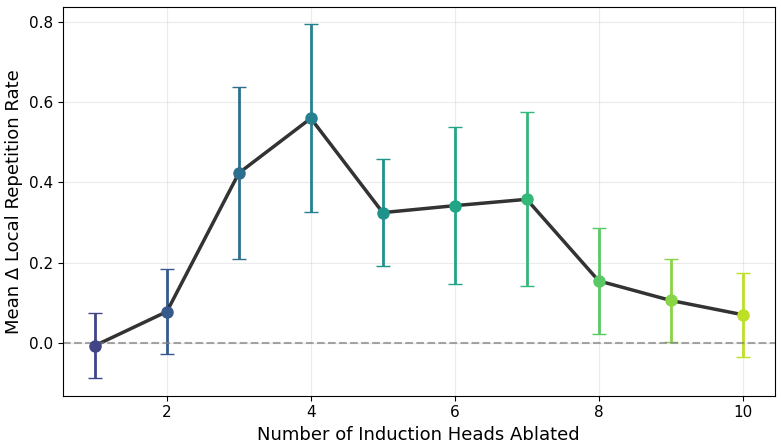
\includegraphics[width=0.78\linewidth]{Figure_4.png}
    \caption{$\Delta$LRR increasing with increasing ablations upto a threshold value, following which it decreased.}
    \label{fig:threshold}
\end{figure}

While this study does not attempt to mechanistically explain this behavior, there are some mechanistic explanations that can explain this behavior. One plausible theory is that ablating induction heads beyond the threshold value leads to a breakdown of the induction circuitry to a point where model output becomes incoherent instead of repetitive. The existence of a non-linear threshold can possibly be explained by the stacking effect used to differentiate the effect of per-head and global ablation. That being said, more rigorous testing will need to be conducted to validate any of these claims. 


\subsection{Generalizing to another Model}

To ensure that local repetition is not only a product of ablating induction heads in small models, the primary result was further validated using the GPT-2 Medium model. This model consists of 355 million parameters as compared to the 124 million parameters in GPT-2 Small \cite{radford2019gpt2}. When the same prompt pipeline and induction-head finding algorithms were applied to this model the $\mu_{\Delta LRR}$ is 0.1853 yielding $p \approx 0.0041$ which remains statistically significant, however the mean differential is not as great as in GPT-2 Small. This result can be explained by the more complex model architecture which leads to suppression of individual mechanistic effects. A similar effect was also noted by Olsson et al with regards to the effect of induction circuits more broadly \cite{olsson2022incontextlearninginductionheads}.

\section{Discussion}

The results shown in this study contribute to existing literature in mechanistic interpretability by proposing a new mechanism by which induction heads prevent model failure. This can potentially help us understand the exact structures in transformers that enable greater performance with scaling, which previous autoregressive models had not been able to show. Additionally, as the field invests more in alignment and AI safety, this study's results might help create more robust fine-tuned models which do not enter repetitive modes. \\

Beyond the primary correlation examined in the study, we also show multiple instances of the non-additive nature of ablation effects. While this is an established result, this study takes the initial observation forward by demonstrating its effect in the context of both final layer entropy and LRR. Another significant finding is the non-linearity in induction head ablation effect, which if observed across model tasks could serve as an important point to consider for future mechanistic interpretability studies and efforts to fine-tune LLMs. However, this study does not have direct implications for improving LLM performance, nevertheless, the insights obtained may play a role in the broader goal of better understanding the inner workings of the model. \\

That being said, there are some limitations of this study which must be acknowledged. Firstly, it's important to point out that the models used in this study (GPT-2 Small and Medium) are toy models and the exact extent to which these findings generalize to frontier models remains unknown. Further, a relatively small number (10) of artificial prompts were used for most experiments in the study due to time and computing constraints; to further make the claims more robust, repetition effects should be tested on a larger number of more natural prompts. \\

Beyond correcting for the limitations of the study, some areas for future study might be to look at attribution scores of non-attention head components in the ablated circuit. While we rigorously examine the role of attention heads with a special focus on induction heads, it might also be worth considering other transformer components like MLPs and how they interact with ablated heads leading to local repetition. Additionally, another scope for future research could be in understanding the mechanistic underpinnings of the non-linear relation obtained to determine causal factors. While not presenting a completely novel pipeline, it is also worth mentioning that the pipeline used in this study presents an easy, multi-step hypothesis generation and verification workflow to examine other LLM behaviors stemming from specific components or circuits.

\section{Conclusion}

This study investigates the effect of induction head ablation on model local repetition using a custom-defined local repetition metric. It further explores the role of final layer entropy and finds an existent but weakly correlated relation with repetition. Local repetition and entropy changes were analyzed under both individual and global head ablation, demonstrating non-additive effects. The original hypothesis was validated through random control ablation and causal activation patching. Additionally, a non-linear relation between local repetition and global induction head ablation was observed, with the primary findings validated on GPT-2 Medium. Overall, the results improve our understanding of the role of induction heads in transformer processes and contribute towards improving LLM interpretability.

\section*{Code Availability}

All code and libraries used are available in the following GitHub Repository: \url{https://github.com/arjun041008/Induction_Head_MechInter}

\bibliographystyle{ieeetr}
\bibliography{references}
\clearpage

\appendix
\onecolumn

\renewcommand{\thefigure}{A.\arabic{figure}}
\renewcommand{\thetable}{A.\arabic{table}}

\setcounter{figure}{0}
\setcounter{table}{0}

\section*{Appendix A: Tables and Figures}

\begin{table}[h]
\centering
\scriptsize
\begin{tabular}{ccc}
\hline
\textbf{Layer} & \textbf{Head} & \textbf{Induction Score} \\
\hline
5  & 5  & 0.8628 \\
5  & 1  & 0.8389 \\
7  & 10 & 0.8350 \\
6  & 9  & 0.7850 \\
7  & 2  & 0.7542 \\
5  & 0  & 0.5168 \\
10 & 7  & 0.4049 \\
8  & 1  & 0.3967 \\
10 & 1  & 0.3893 \\
9  & 9  & 0.3119 \\
\hline
\end{tabular}
\caption{Top induction heads identified in GPT-2 Small ranked by induction score.}
\label{tab:appendix_induction_heads}
\end{table}

\vspace{30pt}

\begin{figure}[h]
\centering
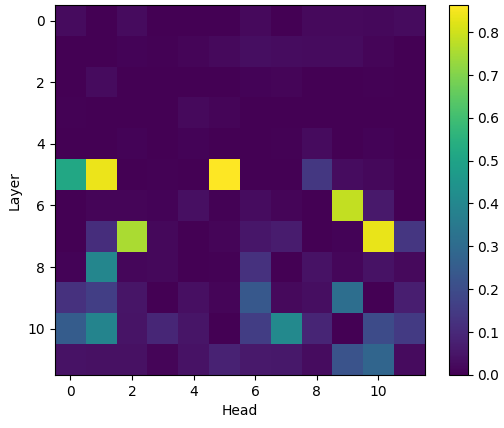
\includegraphics[width=0.42\linewidth]{Figure_5.png}
\caption{Heatmap representing the Induction Score of the various Attention Heads across Layers in GPT-2 Small. Middle layers have the strongest induction scores.}
\label{fig:heatinduc}
\end{figure}

\vspace{40pt}

\begin{table*}[h]

\centering
\scriptsize
\setlength{\tabcolsep}{2pt}

\resizebox{\textwidth}{!}{

\begin{tabular}{p{5.3cm}cccc}

\hline

\textbf{Prompt}
&
\textbf{Clean LRR}
&
\textbf{Ablated LRR}
&
\textbf{Patched LRR}
&
\textbf{Recovery}

\\

\hline

The capital of India is
&
0.2093
&
0.6744
&
0.1512
&
1.1250

\\

The largest planet in the solar system is
&
0.1461
&
0.8090
&
0.1011
&
1.0678

\\

Once upon a time there was
&
0.0805
&
0.3448
&
0.1379
&
0.7826

\\

In a distant galaxy humanity discovered
&
0.1739
&
0.4023
&
0.1149
&
1.2582

\\

The reason climate change is difficult to solve is
&
0.1316
&
0.7889
&
0.1667
&
0.9466

\\

Artificial intelligence may become dangerous if
&
0.0909
&
0.3523
&
0.1250
&
0.8696

\\

Alice went to Paris. Bob went to London. Alice went to
&
0.1489
&
0.6489
&
0.2660
&
0.7660

\\

The cat sat on the mat. The dog sat on the
&
0.1720
&
0.5054
&
0.1935
&
0.9355

\\

The true meaning of life is
&
0.1264
&
0.3678
&
0.1149
&
1.0476

\\

Materialistic Wealth is not sufficient
&
0.0460
&
0.2759
&
0.0805
&
0.8500

\\

\hline

\end{tabular}

}

\caption{
Activation patching results showing Local Repetition Rate (LRR) recovery after patching global induction head activations into the ablated model.
}

\label{tab:activation_patching_results}

\end{table*}

\begin{figure}[t]
\centering
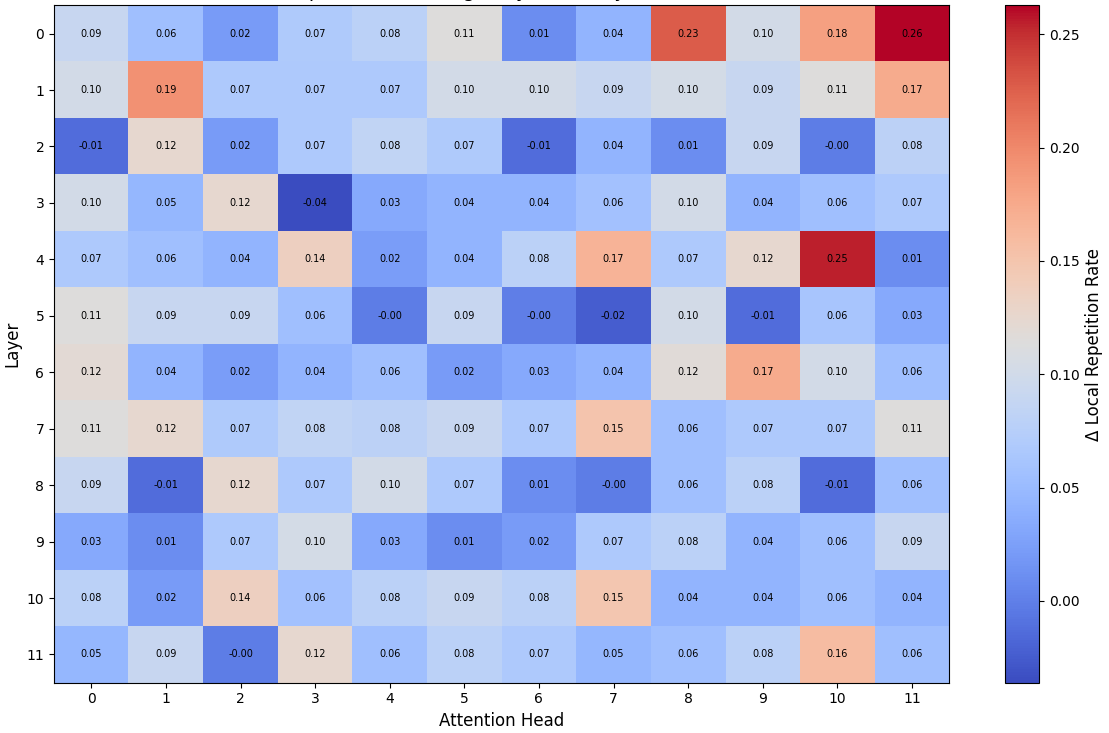
\includegraphics[width=0.42\linewidth]{Figure_6.png}
\caption{$\Delta LRR$ computed by individually ablating heads for the prompt \texttt{"In a distant galaxy humanity discovered"}.}
\label{fig:lrr_appendix}
\end{figure}




\begin{table}

\centering

\scalebox{1.05}{

\begin{tabular}{ccc}

\hline

\textbf{Layer}
&
\textbf{Head}
&
\textbf{Induction Score}

\\

\hline

11 & 1  & 0.8572 \\
9  & 9  & 0.8492 \\
12 & 1  & 0.7873 \\
7  & 2  & 0.7732 \\
6  & 1  & 0.7685 \\
13 & 14 & 0.7116 \\
18 & 5  & 0.6717 \\
5  & 8  & 0.6504 \\
10 & 1  & 0.5020 \\
20 & 7  & 0.4873 \\

\hline

\end{tabular}

}

\caption{
Top induction heads identified in GPT-2 Medium ranked by induction score.
}

\label{tab:appendix_induction_heads_medium}

\end{table}

\begin{algorithm}[t]

\scriptsize

\setlength{\abovedisplayskip}{3pt}
\setlength{\belowdisplayskip}{3pt}

\caption{Identification of Top Induction Heads}

\label{alg:induction_head_identification}

\begin{algorithmic}[1]

\Require Transformer model $M$, sequence length $L$, number of random sequences $N$

\State Initialize score matrix $S \leftarrow 0$

\For{$i=1$ to $N$}

\State Generate random token sequence:

\[
x=[t_1,t_2,\dots,t_L]
\]

\State Duplicate sequence:

\[
x'=[x,x]
\]

\State Run model on $x'$

\ForAll{attention heads $(l,h)$}

\State Obtain attention matrix:

\[
A^{(l,h)}
\]

\State Compute induction score:

\[
I^{(l,h)}
=
\frac{1}{L}
\sum_{i=1}^{L}
A^{(l,h)}_{L+i,i}
\]

\State Update:

\[
S^{(l,h)}
\leftarrow
S^{(l,h)}
+
I^{(l,h)}
\]

\EndFor

\EndFor

\State Normalize:

\[
S\leftarrow S/N
\]

\State Rank attention heads by induction score

\State Return top-$k$ induction heads

\end{algorithmic}

\end{algorithm}

\end{document}

\end{document}